\chapter{Torch implementation take-aways 2}\label{sec:Torch implementation 2}



%
%
% ---- GP-VAE ---------------------------------
%
%

\begin{landscape}
    
\begin{figure}
\begin{centering}
\begin{tikzpicture}[
    % format
    scale=0.55,
    every node/.style={scale=0.55},
    torch/.style={
        rectangle, 
        minimum size=6mm, 
        thick, 
        draw=green!100, 
        fill=green!20, 
        font=\ttfamily
        },
    math/.style={
        rectangle, 
        rounded corners, 
        thick, 
        draw=blue!100,
        fill=blue!20,
        align=center,
        anchor=center,
        inner sep=5pt
        },
    point/.style={
        circle,
        inner sep=0pt,
        minimum size=0pt,
        }
    ]
    % place nodes
    \matrix[row sep = 1mm, column sep=5mm] {
    % row 1
        \node[math] (xt) {
        $\begin{array}{c}
                x_{t_1:t_T} \\
                (B,T,D_x)
        \end{array}$
        }; & 
        \node[torch] (encoder) {
        $\begin{array}{c}
            \text{\ttfamily{Encoder MLP}} \\
            + \, \text{\ttfamily{torch.permute}}
        \end{array}$
        }; &
        \node[math] (zt_perm) {
        $\begin{array}{c}
                z_{t_1:t_T} \\
                (B,D_z,T)
        \end{array}$
        }; & 
        \node[math] (phi) {
            $\begin{array}{c}
                    \mu_{\phi}^l(x_{t_1:t_T}) \,\,\, (B,D_z,T)\\
                    \Sigma_{\phi}^l(x_{t_1:t_T}) \,\,\, (B,D_z,T,T) \\
                    l=1,...,D_z
            \end{array}$
        }; & 
        \node[math] (q_phi) {
        $\begin{array}{c}
        q_{\phi}^l(z_{t_1:t_T} \vert x_{t_1:t_T} ) \\
        (B,D_z) \times \mathcal{N}(T, T\times T)
        \end{array}$
        }; &
        \node[torch] (sample) {
        $\begin{array}{c}
        \text{\ttfamily{Sample}} \\
        + \, \text{\ttfamily{torch.permute}}
        \end{array}$
        }; &
        \node[math] (zt_tilde_perm) {
        $\begin{array}{c}
                \tilde{z}_{t_1:t_T} \\
                (B,T,D_z)
        \end{array}$
        }; & 
        \node[torch] (decoder) {Decoder MLP}; &
        \node[math] (theta_x) {
            $\begin{array}{c}
                    \mu_{\theta_x}^t(z_{t_1:t_T}) \,\,\, (B,T,D_x)\\
                    \Sigma_{\theta_x}^t(z_{t_1:t_T}) \,\,\, (B,T,D_x,D_x) \\
                    t=1,...,T
            \end{array}$
        }; & 
        \node[math] (p_theta_x) {
        $\begin{array}{c}
        p_{\theta_x}(x_{t_1:t_T} \vert \tilde{z}_{t_1:t_T} ) \\ 
        (B,T) \times \mathcal{N}(D_x, D_x\times D_x) \\
        \end{array}$
        }; & \\
    % row 2
    \node[math] (times) {
        $\begin{array}{c}
                {t_1:t_T} \\
                (B,T,1)
        \end{array}$
        }; & &  
    \node[torch] (prior) {GP Prior}; &
    \node[math] (theta_z) {
            $\begin{array}{c}
                    m_{\theta_z, l}({t_1:t_T}) \,\,\, (B,D_z,T)\\
                    k_{\theta_z, l}({t_1:t_T,t_1:t_T}) \,\,\, (B,D_z,T,T) \\
                    l=1,...,D_z
            \end{array}$
        }; &  
    \node[math] (p_theta_z) {
        $\begin{array}{c}
        p_{\theta_z}({t_1:t_T}) \\ 
        (B,D_z) \times \mathcal{N}(T, T\times T) \\
        \end{array}$
        }; & \\
    };
    % draw edges
    \path   (xt) edge [->, thin] (encoder)
            (encoder) edge [->, thin] (zt_perm)
            (zt_perm) edge [->, thin] (phi)
            (phi) edge [->, thin] (q_phi)
            (q_phi) edge [->, thin] (sample)
            (sample) edge [->, thin] (zt_tilde_perm)
            (zt_tilde_perm) edge [->, thin] (decoder)
            (decoder) edge [->, thin] (theta_x)
            (theta_x) edge [->, thin] (p_theta_x)
            (times) edge[->, thin] (prior)
            (prior) edge[->, thin] (theta_z)
            (theta_z) edge[->, thin] (p_theta_z);
\end{tikzpicture}

% --- Loss GPVAE
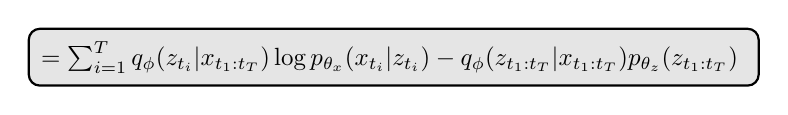
\begin{tikzpicture}[
    scale=0.90,
    every node/.style={scale=0.90},
    math/.style={
        rectangle, 
        % minimum height=1cm,
        % minimum width=2cm,
        rounded corners, 
        thick, 
        draw=black!100,
        fill=gray!20,
        align=center,
        anchor=center,
        inner sep=5pt
        },
    ]
    \node[math] {
        $\VLB = \sum_{i=1}^T \E{q_{\phi}(z_{t_i} \vert x_{t_1:t_T})} \log{p_{\theta_x}(x_{t_i} \vert z_{t_i})} - \KL{q_{\phi}(z_{t_1:t_T} \vert x_{t_1:t_T})}{p_{\theta_z}(z_{t_1:t_T})}$
    };
\end{tikzpicture}

\caption{Gaussian Process VAE Model Architecture}
\end{centering}
\end{figure}

\end{landscape}

         